\Subsection{Prototipo Nido-Sustrato}
Para la construcción del prototipo del nido se tuvo en cuenta que el sustrato sea madera, y que las medidas coincidan con las medias tomadas del paper \cite{ref:varepsilon_madera}, adicionalmente se contempla un lugar donde apoyar la electrónica en el nido, y el hueco de entrada del carpintero.
El diseño del prototipo de nido, se puede observar en los planos especificados en (\ref{fig:base_nido_plano}), (\ref{fig:tapa_nido_plano}) y (\ref{fig:explotado_nido_plano}).

\Subsection{Prototipo Nido-Electrónica}

\Subsubsection{Raspberry Pi}
Para el prototipo se utiliza una Raspberry Pi 3B, sobre la cual se desarrollan los drivers para comunicación con los diversos sensores. Además se desarrolla un \textit{shield}  donde se realiza el acondicionamiento de las señales e interfaz para la placa de sensores.

\begin{figure}[H]
	\centering
	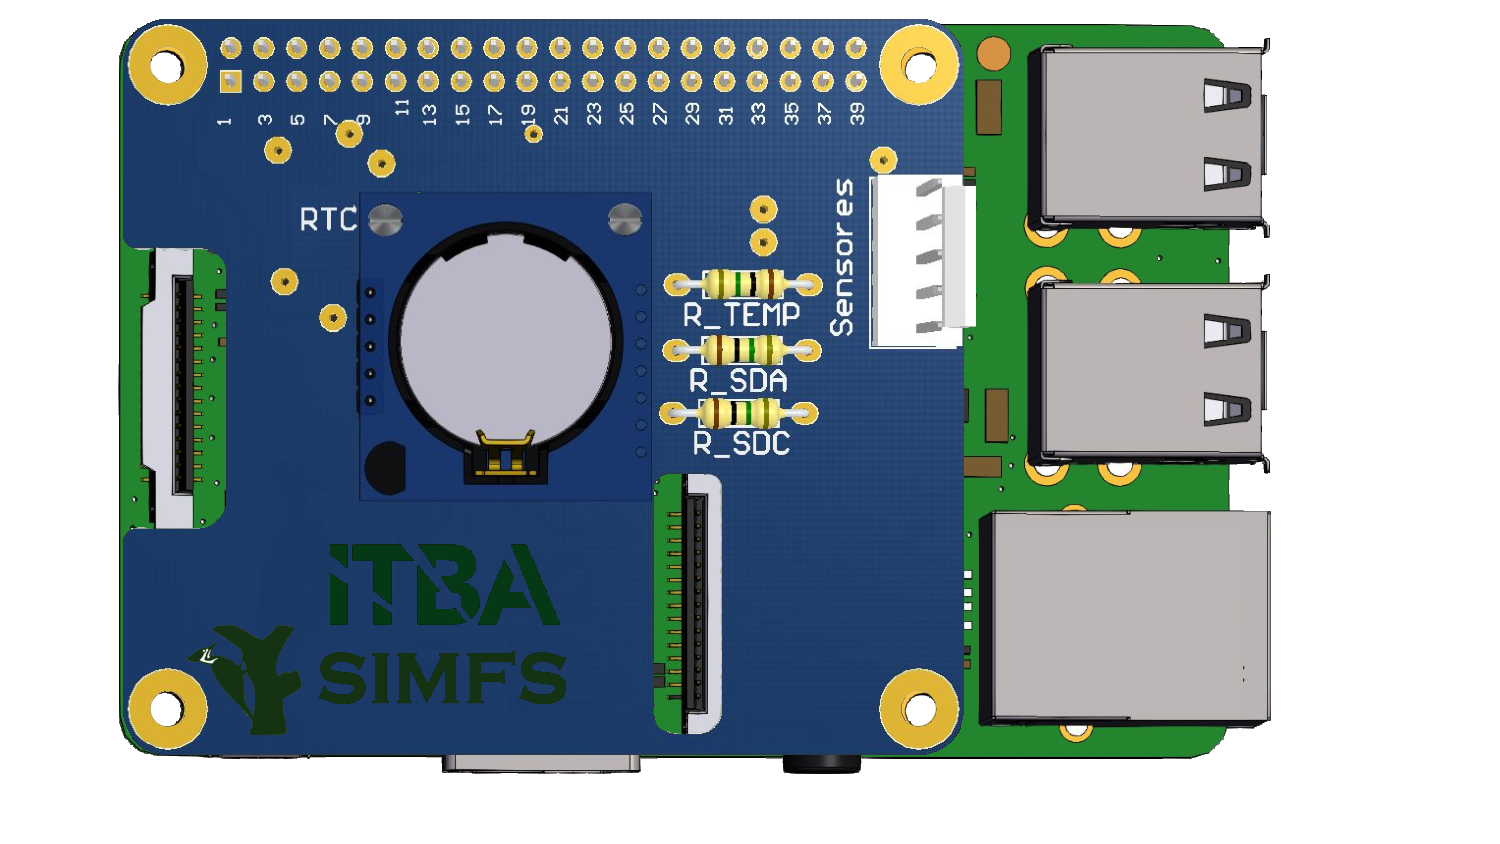
\includegraphics[width=0.9\linewidth,page=1]{ImagenesConstruccion del prototipo/shieldSensor}		
	\caption{Shield  y raspberry pi.}
	\label{fig:shield}
\end{figure}

\Subsubsection{Sensores}
En cuanto a los sensores se diseña una placa que se ubica en la bóveda del nido, la cual nucela todos los sensores necesarios, y ofrece una interfaz con la placa \textit{shield}.
\begin{figure}[H]
	\centering
	\includegraphics[width=0.9\linewidth,page=2]{ImagenesConstruccion del prototipo/shieldSensor}		
	\caption{Placa de sensores.}
	\label{fig:sens}
\end{figure}
\Subsection{Prototipo Nido-Potencia}
Para el prototipo del sistema de potencia del nido, se cuenta con la batería \TBC y la fuente simuladora de paneles solares \TBC.

\Subsection{Prototipo Nido-Comunicaciones }
Existen dos comunicaciones en el prototipo, la encargada de Node-Red para comunicación con usuarios, y la comunicación con la base principal de seguimiento para recolección de datos del ave.
